\documentclass[t,
10pt,
handout, % comment out for getting non handout version
]{beamer}

%beamer settings
\setbeamerfont{normal text}{size=\large}
\AtBeginDocument{\usebeamerfont{normal text}}

% general language
\usepackage{polyglossia}
\setmainfont{Arial}
\setdefaultlanguage{english}
%\usepackage[utf8]{inputenc} % ignor1 anyway due to uft8 based engines
\usepackage[autostyle=true]{csquotes}
\setcounter{tocdepth}{3}
\renewcommand{\baselinestretch}{1.0}

%colors
\usepackage{xcolor}
\definecolor{bluei}{rgb}{0.0, 0.0, 1.0}
\definecolor{greni}{rgb}{0.3, 0.8, 0.2}
\definecolor{greyi}{rgb}{0.5, 0.5 0.5}
\definecolor{b1}{rgb}{0, 0, 0}
\definecolor{r1}{rgb}{255, 0, 0}

% graphics
\usepackage{amssymb}
\usepackage{graphicx}
\usepackage{subfigure}
\usepackage{subcaption}

%date
\usepackage[nodayofweek,level]{datetime}

%change
\newcommand{\authorName}{Janis Jacobi\\Niels Schröter}
\newcommand{\topicName}{physics modelling agent}
\newdate{date1}{24}{12}{2025}

% general layout settings for beamer
\usetheme{Madrid}
%\usecolortheme[RGB={0, 100, 250}]{beamer color theme}
\usecolortheme{seahorse}
%\usefonttheme{structurebold}

\useoutertheme{default}
% beamer template
\setbeamercolor{footline left}{bg=blue!20, fg=b1}
\setbeamercolor{footline center}{bg=blue!10, fg=b1}
\setbeamercolor{footline right}{bg=blue!20, fg=b1}
\setbeamertemplate{footline}{%
	\leavevmode%
	\hbox{%
		\begin{beamercolorbox}[wd=.33\paperwidth,ht=2.5ex,dp=1ex,left]{footline left}%
			\hspace{1em}\topicName
		\end{beamercolorbox}%
		\begin{beamercolorbox}[wd=.34\paperwidth,ht=2.5ex,dp=1ex,center]{footline center}%
			\insertshortdate{}
		\end{beamercolorbox}%
		\begin{beamercolorbox}[wd=.33\paperwidth,ht=2.5ex,dp=1ex,right]{footline right}%
			\insertframenumber{} / \inserttotalframenumber\hspace{1em}
		\end{beamercolorbox}%
	}%
}

\setbeamertemplate{headline}{}
% restore visible bullets



% title-page settings
\title{\topicName}
\subtitle{first prototype}
\date{\today}
%\logo{logo text}
\author{\authorName}

\usepackage[backend=biber, style=numeric, citestyle=numeric, hyperref=true, date=short, backref=false]{biblatex}
%\bibliography{biblio/jabRef.bib}
%\addbibresource{/biblio/jabRef.bib}
\setlength\bibitemsep{7pt}
\setcounter{biburllcpenalty}{9000}

%captions
\usepackage{caption}
\usepackage{subcaption}

%math
\usepackage{mathtools}
\usepackage{unicode-math}
\setmathfont{Latin Modern Math}
\usepackage{amsmath,amssymb}
\usepackage[locale=DE, separate-uncertainty=true]{siunitx}
\usepackage{nicefrac}
\usepackage{physics}
\newcommand{\RNum}[1]{\uppercase\expandafter{\romannumeral #1\relax}} %roman numeral
\numberwithin{equation}{section}
\usepackage{numprint}
\usepackage[version=4]{mhchem}

\newcommand{\al}{\ensuremath{\mathcolor{c1}{|}}}
\newcommand{\scProd}[2]{\ensuremath{\langle #1,#2 \rangle}}
\newcommand{\parti}[2]{\ensuremath{\frac{\mathrm{d}#1}{\mathrm{d}#2}}}
\newcommand{\pard}[2]{\ensuremath{\frac{\partial #1}{\partial #2}}}

% graphics
\usepackage{graphicx}
%\usepackage[margin=2cm]{geometry}
\usepackage{subcaption}
\captionsetup{compatibility=false}

%circuits and drawing
\usepackage{tikz}
\usetikzlibrary{
	shapes.geometric,
	arrows.meta,
	positioning,
	fit,
	calc
}

% insert documents
\usepackage{pdfpages}
\usepackage{float}

% tables
\usepackage{tabularx}
\usepackage{booktabs}
\usepackage{longtable}
\usepackage{pgfplotstable}
\usepackage{multirow}

%csv
\usepackage{csvsimple}

%code
\usepackage{listings}
\usepackage{lstautogobble}
\lstdefinestyle{py}{language={Python}}
\lstset{style=py,
	basicstyle=\normalsize,
	frame=tb,
	language=Python,
	breaklines=true,
	showstringspaces=false,
	columns=flexible,
	stringstyle = \color{blue},
	commentstyle = \color{grey},
	tabsize=3,
	numbers=left,
	keywordstyle=\color{r1},
	columns=flexible,
	frame=single,
	xleftmargin = 20pt,
	autogobble=true,
}

% beamer content display settings:
\usepackage{overpic}

%BIBLIOGRAPHIE
\usepackage[
	backend=biber, %type of file
	style=numeric, %bib entry listing
	citestyle=numeric, % how citation is in text
	hyperref=true, %link the bib entryies
%	date=short, %date format
%	backref=true, % where citation was used
%	url=true, %display url
%	doi=true, % digital object identifier: a permanent, unique link
%	maxbibnames=10, %max number of names displayed
%	minbibnames=3, %minimal number of names displayed
]{biblatex}

\addbibresource{bib/bibliography.bib}
\setlength\bibitemsep{7pt} %spacing between entries
\setcounter{biburlucpenalty}{9000} %prevent mid word url breaks
\setcounter{biburllcpenalty}{9000} %makes sure urls do not run out of the page

%hyperlinks
\usepackage{hyperref}
\hypersetup{
	baseurl={https://www.janisjacobi.de/home.html},
	pdfpagemode = UseNone,
	pdfauthor={\authorName},
	pdfsubject = {\topicName},
	pdfcreator = {\authorName},
	pdfcreationdate = {\today},
	pdfnewwindow,
	bookmarksopen=true,
	backref=page,
	colorlinks,
	urlcolor=bluei,
	citebordercolor=bluei,
	citecolor=bluei,
	linkcolor=bluei,
}

\begin{document}
	\begin{frame}
		\titlepage
	\end{frame}
	
	\begin{frame}{outline}
		\tableofcontents
	\end{frame}
	
	\section{goal of the project \& aim of this prototype}
	
	\begin{frame}[b]{the general goal}
		
		\begin{block}{goal}
			\textit{The \enquote{physics modelling agent} takes a research request as input and suggest a model which answers the research question}
		\end{block}
		\pause
		\begin{alertblock}{how to accomplish that}
			\centering
			\begin{tikzpicture}[
				box/.style={
					align=center,
					rectangle, draw,
					rounded corners,
					minimum width=4cm,
					minimum height=0.8cm,
					align=center,
					fill=blue!20,      % box background color
					text=blue!50!black
				}
				]
				
				\node[box] (n1) {Find relevant sources};
				\pause
				\node[box, below=0.4cm of n1, xshift=2.0cm] (n2) {Extract important info from the sources};
				\draw[->] (n1) -- (n2);
				\pause
				\node[box, below=0.4cm of n2, xshift=2.0cm] (n3) {describe a model to answer the question};
				\draw[->] (n2) -- (n3);
				\pause
				\node[box, below=0.4cm of n3, xshift=2.0cm] (n4) {Create a numerical implementation};
				\draw[->] (n3) -- (n4);
			\end{tikzpicture}
		\end{alertblock}
	\end{frame}
	
	\begin{frame}[c]{this prototype}
		\bigskip
		\begin{minipage}{0.48 \linewidth}
			\centering
			\begin{exampleblock}{what matches the final goal}
				\begin{itemize}
					\item automatically finds real sources
					\item uses the information from these sources
					\item describes a reasonable model
					\item produces easy to execute code
				\end{itemize}
			\end{exampleblock}
		\end{minipage}
		\hfill%
		\pause
		\begin{minipage}{0.48 \linewidth}
			\centering
			\begin{alertblock}{what is still missing}
				\begin{itemize}
					\item the python file does not execute right away
					\item the units of the implementation are wrong
					\item no bench marking yet
					\item no feedback inside the pipeline yet
					\item parameters have not been tweaked yet
				\end{itemize}
			\end{alertblock}
		\end{minipage}
	\end{frame}
	
	
	\section{architecture}
	
	\subsection{constraints}
	
	\begin{frame}[b]{architectural foundations}
		\begin{alertblock}{constraints}
			\begin{itemize}
				\pause
				\item only use open source software
				\item try to use only free software (no payed subscriptions)
			\end{itemize}
		\end{alertblock}
		\pause
		\begin{block}{design choices}
			\begin{itemize}
				\item use SAIA from GWDG\autocite{saiaDoc}
				\begin{itemize}
					\item we have a valid API key for research purposes \autocite{academicId}
				\end{itemize}
				\pause
				\item use an existing framework
				\begin{itemize}
					\item do not re-implement the entire logic for how to orchestrate different AI's
					\item modify the parameters of existing frameworks to get the desired results
				\end{itemize}
			\end{itemize}
		\end{block}
		\pause
		\begin{figure}[h]
			\centering
			
\includegraphics[scale= 0.2]{data/crewAiLogo.png}
			\caption{crewai logo \autocite{crewAi}}
			\label{logoCrewAi}
		\end{figure}
	\end{frame}
	
	\subsection{crewai}
	
	\begin{frame}[b]{crewai: core components}
		\begin{block}{Agents\autocite{agentPy}}
			accesses a LLM to work on a given topic
			\pause
			\begin{itemize}
				\item accesses the LLM via specific object (allows to use SAIA or any other provider, specifies which model to use)
				\item behaviour can be defined via parameters (name, goal, backstory, temperature)
				\item tools can be added to allow advanced abilities (web search, code execution)
			\end{itemize}
		\end{block}
		\pause
		\begin{block}{Tasks\autocite{taskPy}}
			describe a concrete action to execute
			\pause
			\begin{itemize}
				\item has task description and expected output parameters
				\item gets an agent object assigned (execution merges agent and task description)
			\end{itemize}
		\end{block}
	\end{frame}
	\begin{frame}[c]{crewai: orchestration}
		\begin{block}{Crew\autocite{crewPy}}
			this puts it all together and orchestrates order of task executions
		\end{block}
		\centering
		\pause
		\begin{tikzpicture}[
			box/.style={
				rectangle, draw, rounded corners,
				minimum width=2.0cm, minimum height=0.8cm,
				align=center, fill=blue!15, font=\normalsize
			},
			smallbox/.style={
				rectangle, draw, rounded corners,
				minimum width=2.0cm, minimum height=0.6cm,
				align=center, fill=blue!10, font=\scriptsize
			},
			arrow/.style={->, thick}
			]
			
			% Main horizontal flow
			\node[box] (input) {input};
			\node[box, right=2cm of input] (crew) {Crew};
			\node[box, right=2cm of crew] (output) {output\\- files\\- text};
			
			\draw[arrow] (input) -- (crew);
			\draw[arrow] (crew) -- (output);
			\pause
			% Internal vertical flow under Crew
			\node[box, below=1.0cm of crew, xshift=-2.0cm] (assemble) {assemble crew};
			\node[box, below=0.8cm of assemble, xshift=-1.5cm] (agents) {initialise agents};
			\node[box, below=0.8cm of assemble, xshift=+1.5cm ] (tasks) {initialise tasks\\ \bullet assign agent};
			\node[box, below=1.0cm of crew, xshift = 2.0cm] (run) {run crew};
			
			\draw[dashed, arrow] (crew) -- (assemble) node[midway, right] {inside crew};
			\draw[dashed, arrow] (run) -- (crew);
			
			\draw[dashed, arrow] (assemble) -- (agents) node[midway, right] {1};
			\draw[dashed, arrow] (assemble) -- (tasks) node[midway, right] {2};
			\draw[dashed, arrow] (assemble) -- (run) node[midway, right] {3};
		\end{tikzpicture}
		
	\end{frame}
	
	\begin{frame}[c]{crews internal logic}
		upon creation of \enquote{crew} object:
		\begin{itemize}
			\item creates agent and task objects from config-files
		\end{itemize}
		\pause
		\centering
		\begin{tikzpicture}[
			box/.style={
				rectangle, draw, rounded corners,
				minimum width=2.8cm, minimum height=0.8cm,
				align=center, fill=blue!15, font=\small
			},
			smallbox/.style={
				rectangle, draw, rounded corners,
				minimum width=2.4cm, minimum height=0.6cm,
				align=center, fill=blue!10, font=\scriptsize
			},
			arrow/.style={->, thick}
			]
			
			% kickoff
			\node[box] (kickoff) {kickoff};
			\pause
			% hierarchical (off to the side)
			\node[smallbox, below=0.6cm of kickoff] (hier) {Hierarchical\\\scriptsize $\bullet$ not chosen\\\scriptsize $\bullet$ for simplicity};
			\draw[arrow] (kickoff) -- (hier);
			
			% sequential (diagonal)
			\node[box, below right=0.7cm and 0.0cm of kickoff, xshift=0.4cm] (seq) {\_run\_sequential\_process};
			
			\draw[arrow] (kickoff) -- (seq);
			\pause
			
			% execute_tasks
			\node[box, below right=0.7cm of seq, xshift=-2.7cm] (exec) {\_execute\_tasks\\$\bullet$ in order of creation\\$\bullet$ accumulate output in task\_outputs\\$\bullet$ pass to next task};
			
			\draw[arrow] (seq) -- (exec);
			\pause
			% create_crew_output
			\node[box, below=0.4cm of exec, xshift=0cm] (out) {crew\_output\\$\bullet$ creates Output object};
			
			\draw[arrow] (exec) -- (out);		
		\end{tikzpicture}
	\end{frame}

	
	\section{example workflow}
	
	\subsection{input}
	\subsection{the Edelstein effect}
	\begin{frame}[c]{example: input/modelling request}
		\begin{exampleblock}{input}
			\Large aim : \enquote{Calculate the Edelstein effect for a Rashba fermion (at the Gamma point of the Brillouin zone). Compute the magnitization magnitude and direction of different directions and magnitudes of the applied electric field. Consider how the result depends on relevant parameters of the model (e.g. chirality, fermi velocity, spin-orbit coupling strength) and make explicit graphics.}\\
			\bigskip
			topic : Edelstein-Effect\\
		\end{exampleblock}
	\end{frame}
	
	\subsection{pipeline}
	
	\begin{frame}[c]{pipeline}
		\centering
		\begin{tikzpicture}[
			stage/.style={
				rectangle, draw, rounded corners,
				minimum width=2.8cm, minimum height=0.6cm,
				align=center, fill=blue!15, font=\small
			},
			sub/.style={
				rectangle, draw, rounded corners,
				minimum width=2.2cm, minimum height=0.5cm,
				align=center, fill=blue!10, font=\scriptsize
			},
			arrow/.style={->, thick}
			]
			
			% ---------------- INPUT ----------------
			\node[stage] (input) {Input};
			
			
			% ---------------- gather ----------------
			\pause
			\node[stage, below=0.5cm of input] (gather) {gather};
			\draw[arrow, red] (input) -- (gather);
			
			\node[sub, right=1.8cm of gather] (t1) {search through Arxiv for relevant papers};
			\draw[arrow, gray] (gather) -- (t1);
			
			% --------------- download ---------------
			\pause
			\node[stage, below=0.5 of gather] (download) {download};
			\draw[arrow, red] (gather) -- (download);
			
			\node[sub, right=1.8cm of download] (t1p5) {download the papers to local a directory};
			\draw[arrow, gray] (download) -- (t1p5);
			
			% ---------------- extract ----------------
			\pause
			\node[stage, below=0.5cm of download] (extract) {extract};
			\draw[arrow, red] (download) -- (extract);
			
			\node[sub, right=1.8cm of extract] (t2) {filter the necessary info from the papers in the directory};
			\draw[arrow, gray] (extract) -- (t2);
			
			% ---------------- model ----------------
			\pause
			\node[stage, below=0.5cm of extract] (model) {model};
			\draw[arrow, red] (extract) -- (model);

			\node[sub, right=1.8cm of model] (t3) {create a model that answers the request};
			\draw[arrow, gray] (model) -- (t3);
			
			% ---------------- simulate ----------------
			\pause
			\node[stage, below=0.5cm of model] (unitCheck) {unit check};
			\draw[arrow, red] (model) -- (unitCheck);
			
			\node[sub, right=1.8cm of unitCheck] (t4) {check the necessary formulas for correct units};
			\draw[arrow, gray] (unitCheck) -- (t4);
			
			% ---------------- check -----------------
			\pause
			\node[stage, below=0.5 of unitCheck] (simulate) {simulate};
			\draw[arrow, red] (unitCheck) -- (simulate);
			
			\node[sub, right=1.8cm of simulate] (t5) {create a numerical simulation of the model};
			\draw[arrow, gray] (simulate) -- (t5);
			
			% ---------------- final output ----------------
%			\pause
%			\node[stage, below=0.5cm of check] (final) {final output};
%			\draw[arrow, red] (check) -- (final);
		\end{tikzpicture}
	\end{frame}
	
	\subsection{agent \& task configuration}
	
	\begin{frame}[c]{gather}
		\begin{minipage}[h]{0.11 \linewidth}
			\begin{tikzpicture}[
				stage/.style={
					rectangle, draw, rounded corners,
					minimum width=1.7cm, minimum height=0.65cm,
					align=center, font=\small
				},
				graybox/.style={
					stage, fill=gray!20
				},
				modelbox/.style={
					stage, fill=blue!20
				},
				arrow/.style={->, thick, black}
				]
				
				% Input
				\node[graybox] (input) {Input};
				
				% gather
				\node[modelbox, below=0.5cm of input] (gather) {gather};
				
				% download
				\node[graybox, below=0.5 of gather] (download) {download};
				
				% extract
				\node[graybox, below=0.5cm of download] (extract) {extract};
				
				% model (highlighted)
				\node[graybox, below=0.5cm of extract] (model) {model};
				
				% simulate
				\node[graybox, below=0.5cm of model] (checkUnits) {unit check};
				
				% final output
				\node[graybox, below=0.5cm of checkUnits] (simulate) {simulate};
				
				% proper arrows between nodes
				\draw[arrow] (input)   -- (gather);
				\draw[arrow] (gather)  -- (download);
				\draw[arrow] (download)  -- (extract);
				\draw[arrow] (extract) -- (model);
				\draw[arrow] (model)   -- (checkUnits);
				\draw[arrow] (checkUnits)-- (simulate);
			\end{tikzpicture}
		\end{minipage}
		\hfill
		\begin{minipage}{0.84\linewidth}
			agent: find relevant scientific papers
			\pause
			\begin{itemize}
				\item temperature = 0.0; no creativity
				\pause
				\item llm-model = qwen3.5-122b-a10b\autocite{qwenteam2026}; large inputs
				\pause
				\item tools = ArxivPaperTool (searches through Arxiv)
			\end{itemize}
			\smallskip
			\pause
			task: list sources containing relevant information
			\begin{itemize}
				\item output\_file: create a markdown file
			\end{itemize}
			\pause
			\begin{figure}
				\centering
				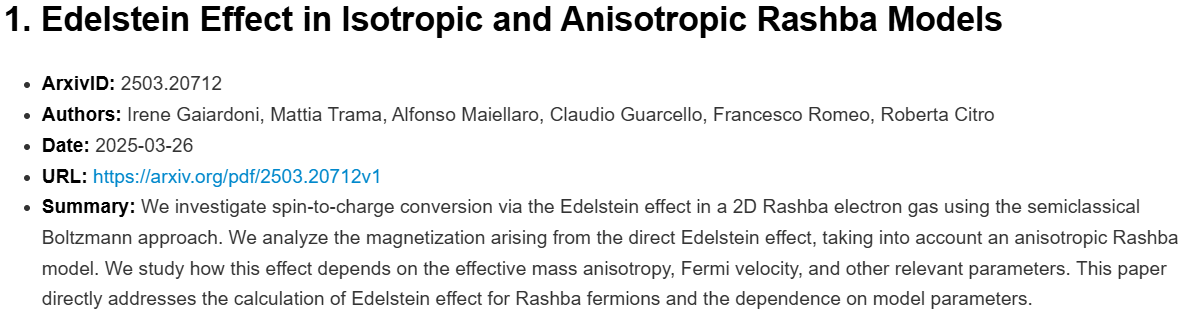
\includegraphics[scale=0.32]{data/gatherOut.png}
				\caption{source gatherer example output}
			\end{figure}
		\end{minipage}
	\end{frame}
	
	\begin{frame}[c]{download}
		\begin{minipage}[H]{0.11 \linewidth}
			\centering
			\begin{tikzpicture}[
				stage/.style={
					rectangle, draw, rounded corners,
					minimum width=1.7cm, minimum height=0.65cm,
					align=center, font=\small
				},
				graybox/.style={
					stage, fill=gray!20
				},
				modelbox/.style={
					stage, fill=blue!20
				},
				arrow/.style={->, thick, black}
				]
				
				% Input
				\node[graybox] (input) {Input};
				
				% gather
				\node[graybox, below=0.5cm of input] (gather) {gather};
				
				% download
				\node[modelbox, below=0.5 of gather] (download) {download};
				
				% extract
				\node[graybox, below=0.5cm of download] (extract) {extract};
				
				% model (highlighted)
				\node[graybox, below=0.5cm of extract] (model) {model};
				
				% simulate
				\node[graybox, below=0.5cm of model] (checkUnits) {unit check};
				
				% final output
				\node[graybox, below=0.5cm of checkUnits] (simulate) {simulate};
				
				% proper arrows between nodes
				\draw[arrow] (input)   -- (gather);
				\draw[arrow] (gather)  -- (download);
				\draw[arrow] (download)  -- (extract);
				\draw[arrow] (extract) -- (model);
				\draw[arrow] (model)   -- (checkUnits);
				\draw[arrow] (checkUnits)-- (simulate);
			\end{tikzpicture}
		\end{minipage}
		\hfill
		\begin{minipage}[c]{0.84\linewidth}
			agent: download papers to local directory \pause
			\begin{itemize}
				\item temperature = 0.0; no creativity
				\item llm-model = qwen3.5-122b-a10b\autocite{qwenteam2026}; large inputs
				\item tools = ArxivDownloader (extends ArxivPaperTool)
			\end{itemize}
			\smallskip\pause
			task: download the papers; report issues\pause
			\begin{figure}
				\centering
				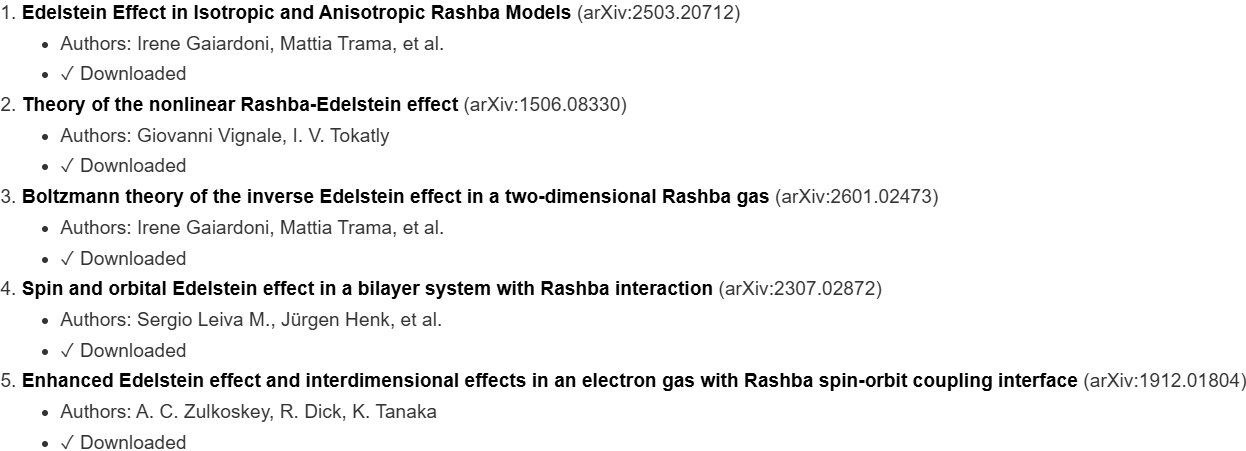
\includegraphics[scale=0.30]{data/download.png}
				\caption{download report}
			\end{figure}
		\end{minipage}
	\end{frame}
	
	\begin{frame}[c]{extract information I}
		\begin{minipage}[h]{0.11 \linewidth}
			\begin{tikzpicture}[
				stage/.style={
					rectangle, draw, rounded corners,
					minimum width=1.7cm, minimum height=0.65cm,
					align=center, font=\small
				},
				graybox/.style={
					stage, fill=gray!20
				},
				modelbox/.style={
					stage, fill=blue!20
				},
				arrow/.style={->, thick, black}
				]
				
				% Input
				\node[graybox] (input) {Input};
				
				% gather
				\node[graybox, below=0.5cm of input] (gather) {gather};
				
				% download
				\node[graybox, below=0.5 of gather] (download) {download};
				
				% extract
				\node[modelbox, below=0.5cm of download] (extract) {extract};
				
				% model (highlighted)
				\node[graybox, below=0.5cm of extract] (model) {model};
				
				% simulate
				\node[graybox, below=0.5cm of model] (checkUnits) {unit check};
				
				% final output
				\node[graybox, below=0.5cm of checkUnits] (simulate) {simulate};
				
				% proper arrows between nodes
				\draw[arrow] (input)   -- (gather);
				\draw[arrow] (gather)  -- (download);
				\draw[arrow] (download)  -- (extract);
				\draw[arrow] (extract) -- (model);
				\draw[arrow] (model)   -- (checkUnits);
				\draw[arrow] (checkUnits)-- (simulate);
			\end{tikzpicture}
		\end{minipage}
		\hfill
		\begin{minipage}{0.84\linewidth}
			agent: extract information using the downloaded papers \pause
			\begin{itemize}
				\item temperature = 0.0; no creativity
				\item llm-model = qwen3.5-122b-a10b\autocite{qwenteam2026}; large inputs
				\item tools = PDFReader (reading pdf from local dir)
			\end{itemize}
			\smallskip\pause
			task: present info that allows building the model
			\begin{figure}
				\centering
				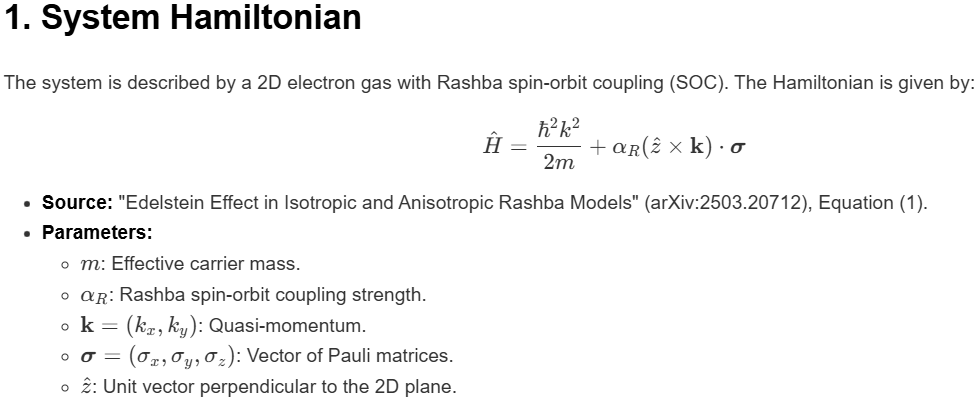
\includegraphics[scale=0.33]{data/info.png}
				\caption{information extractor example output}
			\end{figure}
		\end{minipage}
	\end{frame}
	
	\begin{frame}[c]{extract information II}
		\begin{minipage}[h]{0.11 \linewidth}
			\begin{tikzpicture}[
				stage/.style={
					rectangle, draw, rounded corners,
					minimum width=1.7cm, minimum height=0.65cm,
					align=center, font=\small
				},
				graybox/.style={
					stage, fill=gray!20
				},
				modelbox/.style={
					stage, fill=blue!20
				},
				arrow/.style={->, thick, black}
				]
				
				% Input
				\node[graybox] (input) {Input};
				
				% gather
				\node[graybox, below=0.5cm of input] (gather) {gather};
				
				% download
				\node[graybox, below=0.5 of gather] (download) {download};
				
				% extract
				\node[modelbox, below=0.5cm of download] (extract) {extract};
				
				% model (highlighted)
				\node[graybox, below=0.5cm of extract] (model) {model};
				
				% simulate
				\node[graybox, below=0.5cm of model] (checkUnits) {unit check};
				
				% final output
				\node[graybox, below=0.5cm of checkUnits] (simulate) {simulate};
				
				% proper arrows between nodes
				\draw[arrow] (input)   -- (gather);
				\draw[arrow] (gather)  -- (download);
				\draw[arrow] (download)  -- (extract);
				\draw[arrow] (extract) -- (model);
				\draw[arrow] (model)   -- (checkUnits);
				\draw[arrow] (checkUnits)-- (simulate);
			\end{tikzpicture}
		\end{minipage}
		\hfill
		\begin{minipage}{0.84\linewidth}
			other key findings: 
			\begin{itemize}
				\item Energy dispwersion: $\epsilon_k^\nu = \frac{k^2}{2m} + \nu k \alpha$ mit $\nu = \pm 1$
				\item High-Density-Regime: ($\mu \geq 0$):
				\begin{itemize}
					\item $k_F^\nu = - \nu k_0 + \sqrt{k_0^2 + 2m\mu}$
					\item $M_y = \frac{\mu_b \abs{e} \tau}{2 \pi} m \alpha \left[\hat{z} \times \bold{E}\right]_y$
				\end{itemize}
				\item Low-Density-Regime: ($\mu < 0$)
				\begin{itemize}
					\item $k_F^\eta =k_0 - \eta \sqrt{k_0^2 + 2m\mu}$
					\item $M_y = \frac{\mu_b \abs{e} \tau}{2 \pi} \sqrt{m^2 \alpha^2 + 2m E_F} \left[\hat{z} \times \bold{E}\right]_y$
				\end{itemize}
				\item parameters:
				\begin{itemize}
					\item chirality $\nu$, in Low-Density-Regime also transport chirality $\eta$
					\item Fermi velocity $v_F$, dependency implicitly via $\alpha$ and $m$
					\item Rashba coupling $\alpha$, for $\alpha \rightarrow 0$ Edelstein effect vanishes
					\item effectice mass $m$, in High-Density-Regime proportional to Magentization $M$
				\end{itemize}
			\end{itemize}
		\end{minipage}
	\end{frame}
	
	\begin{frame}[c]{model}
		\begin{minipage}{0.11 \linewidth}
			\begin{tikzpicture}[
				stage/.style={
					rectangle, draw, rounded corners,
					minimum width=1.7cm, minimum height=0.65cm,
					align=center, font=\small
				},
				graybox/.style={
					stage, fill=gray!20
				},
				modelbox/.style={
					stage, fill=blue!20
				},
				arrow/.style={->, thick, black}
				]
				
				% Input
				\node[graybox] (input) {Input};
				
				% gather
				\node[graybox, below=0.5cm of input] (gather) {gather};
				
				% download
				\node[graybox, below=0.5 of gather] (download) {download};
				
				% extract
				\node[graybox, below=0.5cm of download] (extract) {extract};
				
				% model (highlighted)
				\node[modelbox, below=0.5cm of extract] (model) {model};
				
				% simulate
				\node[graybox, below=0.5cm of model] (checkUnits) {unit check};
				
				% final output
				\node[graybox, below=0.5cm of checkUnits] (simulate) {simulate};
				
				% proper arrows between nodes
				\draw[arrow] (input)   -- (gather);
				\draw[arrow] (gather)  -- (download);
				\draw[arrow] (download)  -- (extract);
				\draw[arrow] (extract) -- (model);
				\draw[arrow] (model)   -- (checkUnits);
				\draw[arrow] (checkUnits)-- (simulate);
			\end{tikzpicture}
		\end{minipage}
		\hfill
		\begin{minipage}{0.84\linewidth}
			agent: build a model that solves the problem \pause
			\begin{itemize}
				\item temperature = 0.0; for reproducibility \pause
				\item llm-model = deepseek-r1-distill-llama-70b\autocite{deepSeek}; reasoning
			\end{itemize}
			\smallskip
			\pause
			task: mathematical description with textual explanation\\\pause
			{\centering
			\color{red}the model reproduces the formulas from the extracted information as seen before}
			\begin{figure} % single legal float
				\centering
%				\begin{minipage}[c]{0.4\textwidth}
%					\centering
%					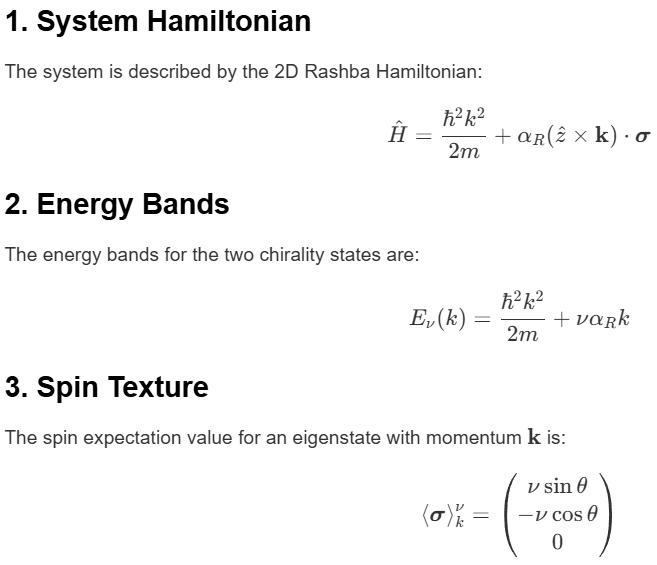
\includegraphics[scale=0.26]{data/model3.png}
%					\captionof{figure}{Modelling example}
%					\label{fig:sub1}
%				\end{minipage}
%				\hfill
%				\begin{minipage}[c]{0.4\textwidth}
%					\centering
%					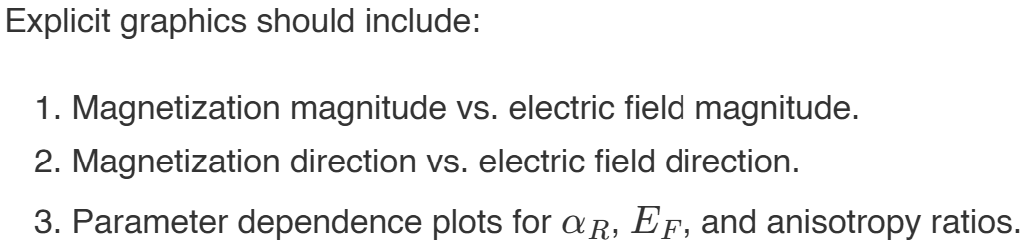
\includegraphics[scale=0.3]{data/model2.png}
%					\captionof{figure}{Parameters}
%					\label{fig:sub2}
%				\end{minipage}
				\centering
				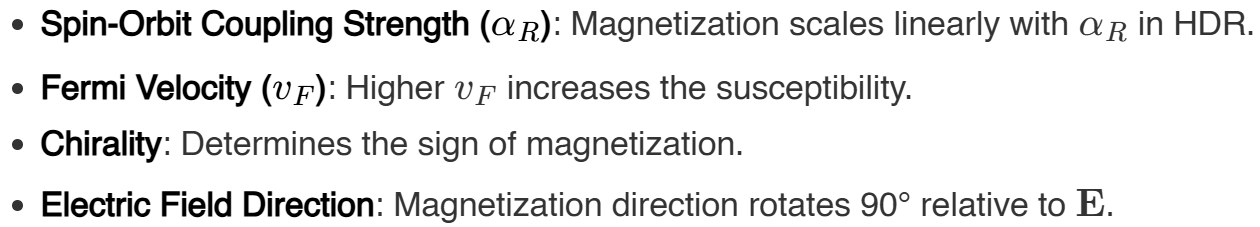
\includegraphics[scale = 0.35]{data/model.png}
				\caption{expected parameter dependencies}
				\pause
				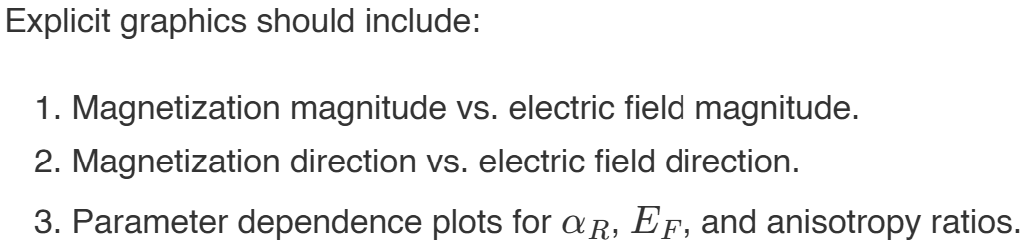
\includegraphics[scale= 0.35]{data/model2.png}
				\caption{planning: which plots should be created}
			\end{figure} 
			
		\end{minipage}
	\end{frame}
	
	\begin{frame}[c]{unit check}
		\begin{minipage}[h]{0.11 \linewidth}
			\begin{tikzpicture}[
				stage/.style={
					rectangle, draw, rounded corners,
					minimum width=1.7cm, minimum height=0.65cm,
					align=center, font=\small
				},
				graybox/.style={
					stage, fill=gray!20
				},
				modelbox/.style={
					stage, fill=blue!20
				},
				arrow/.style={->, thick, black}
				]
				
				% Input
				\node[graybox] (input) {Input};
				
				% gather
				\node[graybox, below=0.5cm of input] (gather) {gather};
				
				% download
				\node[graybox, below=0.5 of gather] (download) {download};
				
				% extract
				\node[graybox, below=0.5cm of download] (extract) {extract};
				
				% model (highlighted)
				\node[graybox, below=0.5cm of extract] (model) {model};
				
				% simulate
				\node[modelbox, below=0.5cm of model] (checkUnits) {unit check};
				
				% final output
				\node[graybox, below=0.5cm of checkUnits] (simulate) {simulate};
				
				% proper arrows between nodes
				\draw[arrow] (input)   -- (gather);
				\draw[arrow] (gather)  -- (download);
				\draw[arrow] (download)  -- (extract);
				\draw[arrow] (extract) -- (model);
				\draw[arrow] (model)   -- (checkUnits);
				\draw[arrow] (checkUnits)-- (simulate);
			\end{tikzpicture}
		\end{minipage}
		\hfill
		\begin{minipage}[h]{0.84\linewidth}
			agent: check formulas and units\pause
			\begin{itemize}
				\item temperature = 0.0; no creativity\pause
				\item llm-model = deepseek-r1-distill-llama-70b\autocite{deepSeek}\pause
				\item use previous work (no tools)
			\end{itemize}
			\smallskip
			task: check the units of the model; correct them if necessary\pause
			\begin{figure} % single legal float
				\centering
				\begin{minipage}[c]{0.4\textwidth}
					\centering
					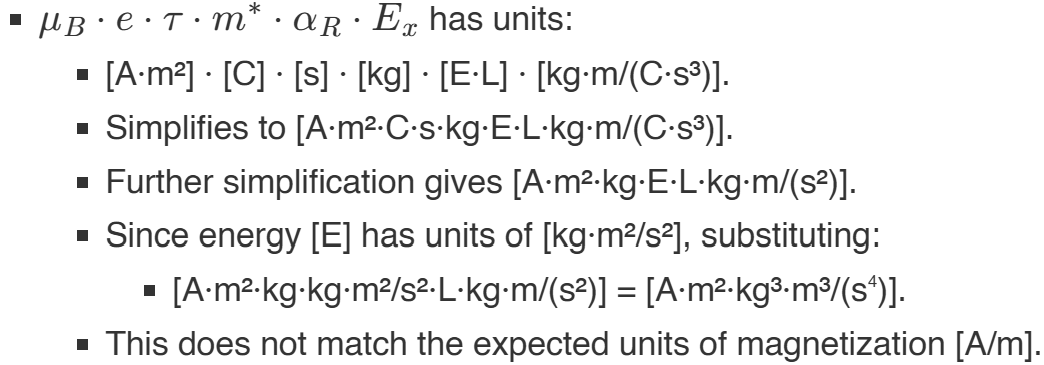
\includegraphics[scale=0.35]{data/units.png}
					\captionof{figure}{unit checks: the unit of the magnetization does not match \si{\ampere \meter}}
					\label{fig:units}
				\end{minipage}\pause
				\hfill
				\begin{minipage}[c]{0.4\textwidth}
					\centering
					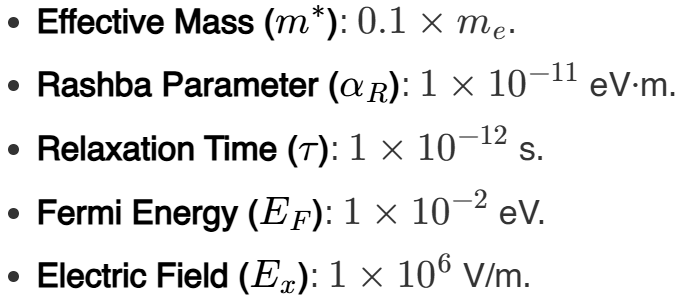
\includegraphics[scale=0.4]{data/startingPrams.png}
					\captionof{figure}{starting parameters}
					\label{fig:params}
				\end{minipage}
			\end{figure} 
		\end{minipage}
	\end{frame}
	
	\begin{frame}[c]{simulation I}
		\begin{minipage}[h]{0.11 \linewidth}
			\begin{tikzpicture}[
				stage/.style={
					rectangle, draw, rounded corners,
					minimum width=1.7cm, minimum height=0.65cm,
					align=center, font=\small
				},
				graybox/.style={
					stage, fill=gray!20
				},
				modelbox/.style={
					stage, fill=blue!20
				},
				arrow/.style={->, thick, black}
				]
				
				% Input
				\node[graybox] (input) {Input};
				
				% gather
				\node[graybox, below=0.5cm of input] (gather) {gather};
				
				% download
				\node[graybox, below=0.5 of gather] (download) {download};
				
				% extract
				\node[graybox, below=0.5cm of download] (extract) {extract};
				
				% model (highlighted)
				\node[graybox, below=0.5cm of extract] (model) {model};
				
				% simulate
				\node[graybox, below=0.5cm of model] (checkUnits) {unit check};
				
				% final output
				\node[modelbox, below=0.5cm of checkUnits] (simulate) {simulate};
				
				% proper arrows between nodes
				\draw[arrow] (input)   -- (gather);
				\draw[arrow] (gather)  -- (download);
				\draw[arrow] (download)  -- (extract);
				\draw[arrow] (extract) -- (model);
				\draw[arrow] (model)   -- (checkUnits);
				\draw[arrow] (checkUnits)-- (simulate);
			\end{tikzpicture}
		\end{minipage}
		\hfill
		\begin{minipage}[h]{0.84\linewidth}
			agent: create a numerical implementation of the model\pause
			\begin{itemize}
				\item temperature = 0.1; even less creative\pause
				\item llm-model = devstral-2-123b-instruct-2512\autocite{huggFace}; coding \pause
			\end{itemize}
			\smallskip
			task: create executable python code
			\begin{figure}[h]
				\centering
				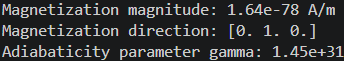
\includegraphics[scale=0.7]{data/simulation_Output.png}
				\caption{calculated magnetisation, wrong by many magnitudes: $M_y = \frac{\mu_B \abs{e} \tau}{2 \pi} n^* \alpha_R E_x$}
				\label{crewSimRes}
			\end{figure}\pause
			The calculation is wrong because of unit mismatches. This is caused by the incomplete formula.
			
			The formula implementation sometimes drops the Bohr Magenton $\mu_B$
			
		\end{minipage}
	\end{frame}
	
	\begin{frame}[c]{simulation II}
		\begin{minipage}{0.11 \linewidth}
			\begin{tikzpicture}[
				stage/.style={
					rectangle, draw, rounded corners,
					minimum width=1.7cm, minimum height=0.65cm,
					align=center, font=\small
				},
				graybox/.style={
					stage, fill=gray!20
				},
				modelbox/.style={
					stage, fill=blue!20
				},
				arrow/.style={->, thick, black}
				]
				
				% Input
				\node[graybox] (input) {Input};
				
				% gather
				\node[graybox, below=0.5cm of input] (gather) {gather};
				
				% download
				\node[graybox, below=0.5 of gather] (download) {download};
				
				% extract
				\node[graybox, below=0.5cm of download] (extract) {extract};
				
				% model (highlighted)
				\node[graybox, below=0.5cm of extract] (model) {model};
				
				% simulate
				\node[graybox, below=0.5cm of model] (checkUnits) {unit check};
				
				% final output
				\node[modelbox, below=0.5cm of checkUnits] (simulate) {simulate};
				
				% proper arrows between nodes
				\draw[arrow] (input)   -- (gather);
				\draw[arrow] (gather)  -- (download);
				\draw[arrow] (download)  -- (extract);
				\draw[arrow] (extract) -- (model);
				\draw[arrow] (model)   -- (checkUnits);
				\draw[arrow] (checkUnits)-- (simulate);
			\end{tikzpicture}
		\end{minipage}
		\hfill
		\begin{minipage}{0.84\linewidth}
			result: \textbf{executable code} \pause
			\begin{itemize}
				\item the general relations match but their magnituedes are useless
			\end{itemize}
			\begin{figure}
				\centering
				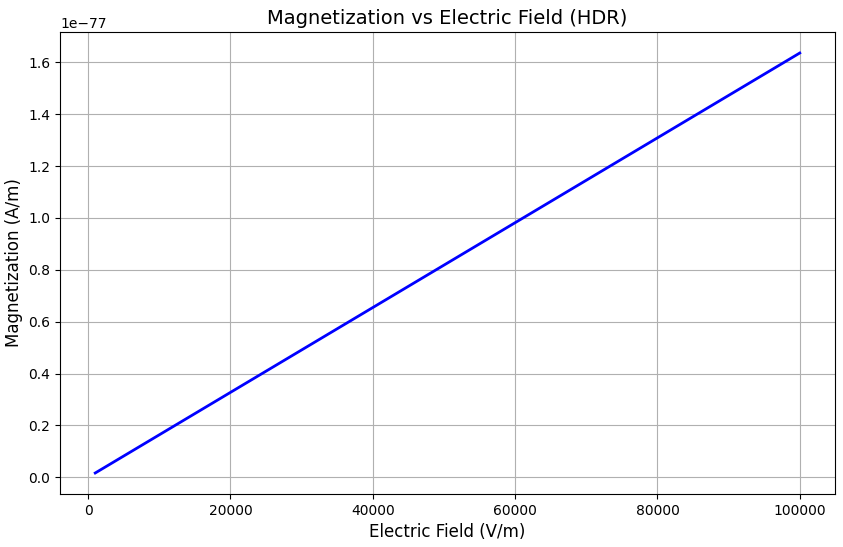
\includegraphics[scale=0.31]{data/magnE.png}
				\caption{Magentization vs. electric Field; linear dependency is expected}
				\label{crewPlot2}
			\end{figure}
		\end{minipage}
	\end{frame}
	
	\begin{frame}[c]{simulation III}
		\begin{minipage}{0.11 \linewidth}
			\begin{tikzpicture}[
				stage/.style={
					rectangle, draw, rounded corners,
					minimum width=1.7cm, minimum height=0.65cm,
					align=center, font=\small
				},
				graybox/.style={
					stage, fill=gray!20
				},
				modelbox/.style={
					stage, fill=blue!20
				},
				arrow/.style={->, thick, black}
				]
				
				% Input
				\node[graybox] (input) {Input};
				
				% gather
				\node[graybox, below=0.5cm of input] (gather) {gather};
				
				% download
				\node[graybox, below=0.5 of gather] (download) {download};
				
				% extract
				\node[graybox, below=0.5cm of download] (extract) {extract};
				
				% model (highlighted)
				\node[graybox, below=0.5cm of extract] (model) {model};
				
				% simulate
				\node[graybox, below=0.5cm of model] (checkUnits) {unit check};
				
				% final output
				\node[modelbox, below=0.5cm of checkUnits] (simulate) {simulate};
				
				% proper arrows between nodes
				\draw[arrow] (input)   -- (gather);
				\draw[arrow] (gather)  -- (download);
				\draw[arrow] (download)  -- (extract);
				\draw[arrow] (extract) -- (model);
				\draw[arrow] (model)   -- (checkUnits);
				\draw[arrow] (checkUnits)-- (simulate);
			\end{tikzpicture}
		\end{minipage}
		\hfill
		\begin{minipage}{0.84\linewidth}
			\begin{figure} % single legal float
				\centering
				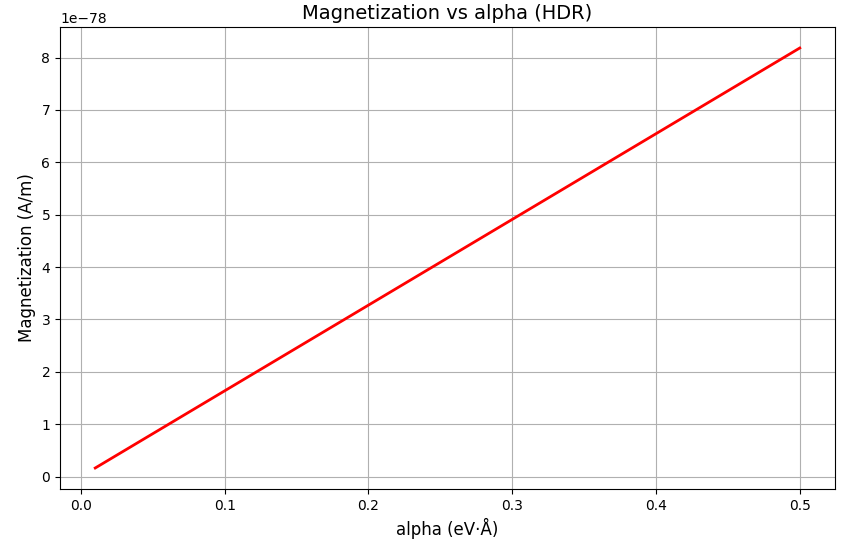
\includegraphics[scale=0.45]{data/magnAlpha.png}
				\captionof{figure}{Magentization vs. Rashba coupling; linear dependency is expected}
				\label{crewPlot4}
			\end{figure}
		\end{minipage}
	\end{frame}
	
	\begin{frame}[c]{simulation IV}
		\begin{minipage}{0.11 \linewidth}
			\begin{tikzpicture}[
				stage/.style={
					rectangle, draw, rounded corners,
					minimum width=1.7cm, minimum height=0.65cm,
					align=center, font=\small
				},
				graybox/.style={
					stage, fill=gray!20
				},
				modelbox/.style={
					stage, fill=blue!20
				},
				arrow/.style={->, thick, black}
				]
				
				% Input
				\node[graybox] (input) {Input};
				
				% gather
				\node[graybox, below=0.5cm of input] (gather) {gather};
				
				% download
				\node[graybox, below=0.5 of gather] (download) {download};
				
				% extract
				\node[graybox, below=0.5cm of download] (extract) {extract};
				
				% model (highlighted)
				\node[graybox, below=0.5cm of extract] (model) {model};
				
				% simulate
				\node[graybox, below=0.5cm of model] (checkUnits) {unit check};
				
				% final output
				\node[modelbox, below=0.5cm of checkUnits] (simulate) {simulate};
				
				% proper arrows between nodes
				\draw[arrow] (input)   -- (gather);
				\draw[arrow] (gather)  -- (download);
				\draw[arrow] (download)  -- (extract);
				\draw[arrow] (extract) -- (model);
				\draw[arrow] (model)   -- (checkUnits);
				\draw[arrow] (checkUnits)-- (simulate);
			\end{tikzpicture}
		\end{minipage}
		\hfill
		\begin{minipage}{0.84\linewidth}
			\begin{figure}
				\centering
				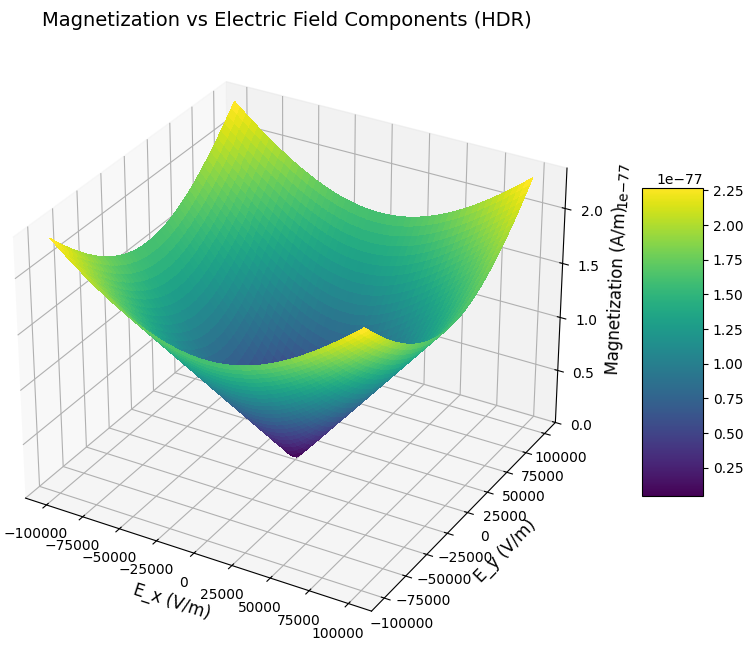
\includegraphics[scale=0.42]{data/magnEField.png}
				\caption{Magentization vs. E-Field in 2D; the relation is correct for the total magnetization}
				\label{crewPlot5}
			\end{figure}
		\end{minipage}
	\end{frame}
	
%	\begin{frame}[c]{{\color{red}update:} validate simulation}
%		\begin{minipage}[h]{0.11 \linewidth}
%			\begin{tikzpicture}[
%				stage/.style={
%					rectangle, draw, rounded corners,
%					minimum width=1.7cm, minimum height=0.65cm,
%					align=center, font=\small
%				},
%				graybox/.style={
%					stage, fill=gray!20
%				},
%				modelbox/.style={
%					stage, fill=blue!20
%				},
%				arrow/.style={->, thick, black}
%				]
%				
%				% Input
%				\node[graybox] (input) {Input};
%				
%				% gather
%				\node[graybox, below=0.5cm of input] (gather) {gather};
%				
%				% download
%				\node[modelbox, below=0.5 of gather] (download) {download};
%				
%				% extract
%				\node[graybox, below=0.5cm of download] (extract) {extract};
%				
%				% model (highlighted)
%				\node[graybox, below=0.5cm of extract] (model) {model};
%				
%				% simulate
%				\node[graybox, below=0.5cm of model] (checkUnits) {unit check};
%				
%				% final output
%				\node[graybox, below=0.5cm of checkUnits] (simulate) {simulate};
%				
%				% proper arrows between nodes
%				\draw[arrow] (input)   -- (gather);
%				\draw[arrow] (gather)  -- (download);
%				\draw[arrow] (download)  -- (extract);
%				\draw[arrow] (extract) -- (model);
%				\draw[arrow] (model)   -- (checkUnits);
%				\draw[arrow] (checkUnits)-- (simulate);
%			\end{tikzpicture}
%		\end{minipage}
%		\hfill
%		\begin{minipage}[h]{0.84\linewidth}
%			agent: check formulas and units\pause
%			\begin{itemize}
%				\item temperature = 0.0; no creativity\pause
%				\item llm-model = deeps\autocite{qwenteam2026}; tool use for unit and parameter choice \pause
%				\item tools = PDFReader (use the papers found)
%			\end{itemize}
%			\smallskip
%			task: check necessary formulas and units for the model implementation
%			\begin{figure}
%				\centering
%				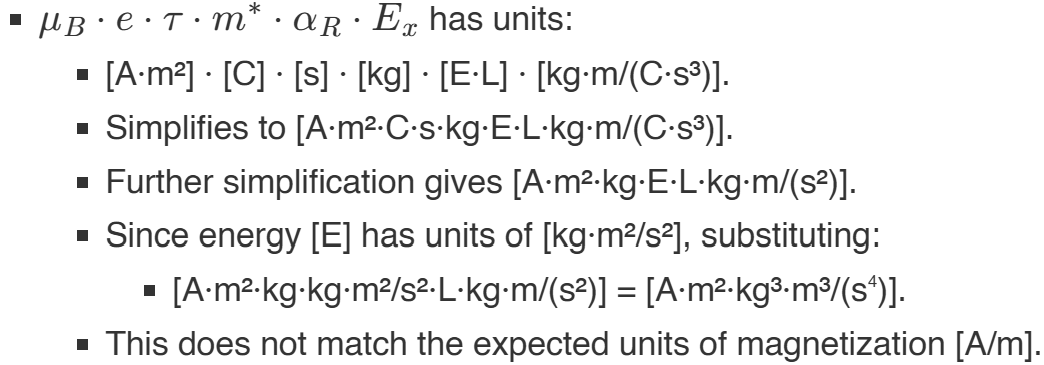
\includegraphics[scale=0.33]{data/units.png}
%				\caption{unit conversions of planning task}
%				\label{validate}
%			\end{figure}
%		\end{minipage}
%	\end{frame}
%	
%	\begin{frame}[c]{check}
%		\begin{minipage}{0.11 \linewidth}
%			\begin{tikzpicture}[
%				stage/.style={
%					rectangle, draw, rounded corners,
%					minimum width=1.7cm, minimum height=0.65cm,
%					align=center, font=\small
%				},
%				graybox/.style={
%					stage, fill=gray!20
%				},
%				modelbox/.style={
%					stage, fill=blue!20
%				},
%				arrow/.style={->, thick, black}
%				]
%				
%				% Input
%				\node[graybox] (input) {Input};
%				
%				% gather
%				\node[graybox, below=0.5cm of input] (gather) {gather};
%				
%				% download
%				\node[modelbox, below=0.5 of gather] (download) {download};
%				
%				% extract
%				\node[graybox, below=0.5cm of download] (extract) {extract};
%				
%				% model (highlighted)
%				\node[graybox, below=0.5cm of extract] (model) {model};
%				
%				% simulate
%				\node[graybox, below=0.5cm of model] (checkUnits) {unit check};
%				
%				% final output
%				\node[graybox, below=0.5cm of checkUnits] (simulate) {simulate};
%				
%				% proper arrows between nodes
%				\draw[arrow] (input)   -- (gather);
%				\draw[arrow] (gather)  -- (download);
%				\draw[arrow] (download)  -- (extract);
%				\draw[arrow] (extract) -- (model);
%				\draw[arrow] (model)   -- (checkUnits);
%				\draw[arrow] (checkUnits)-- (simulate);
%			\end{tikzpicture}
%		\end{minipage}
%		\hfill
%		\begin{minipage}{0.84linewidth}
%			agent: compare model results against literature\pause
%			\begin{itemize}
%				\item temperature = 0.0; just compare
%				\item llm-model = qwen3.5-122b-a10b\autocite{qwenteam2026}; good overall
%				\item tools = ArxivDownloader, ArxivPaperTool, PDFReader
%			\end{itemize}\pause
%			task: compare the model and evaluate performance
%			\begin{figure}
%				\centering
%				\includegraphics[scale=0.34]{data/check1.png}
%				\caption{Electric field dependence; simulation plot}
%				\label{check}
%			\end{figure}
%		\end{minipage}
%	\end{frame}
	
	\section{results}
	
	\subsection{parameter choice}
	
	\begin{frame}[c]{parameter choice I: temperature \& models}
		\begin{block}{temperature - creativity of output (0.0 to 1.0)}
			\begin{itemize}
				\item keep at 0.0 if the agent should only find or extract content
				\item{$\rightarrow$} minimise hallucination
				\item allow some creativity for tasks requiring "thought": model making and coding
				\item {\color{blue}future}: test how temperature configuration affects the output 
			\end{itemize}
		\end{block}
		\pause
		\begin{block}{models}
			there is no general benchmark for all SAIA models
			\begin{itemize}
				\item for reasoning tasks use deep-seek models (benchmark: \autocite{deepSeek})
				\item for coding tasks use devstral (no scientific benchmark, github community \enquote{benchmark} at \autocite{huggFace})
				\item for more general tasks use overall strong model qwen3.5 (benchmark \autocite{qwenteam2026})
			\end{itemize}
		\end{block}
	\end{frame}
	
	\begin{frame}[c]{parameter choice II: tools}
		tools enhance an agents capabilities
		\pause
		\begin{block}{ArxivPaperTool}
			\begin{itemize}
				\item crewai provided; finds papers and can read their metadata
				\item can not directly access the PDF contents or download them
				\item used for finding papers
				\end{itemize}
		\end{block}
		\pause
		\begin{block}{ArxivDownloader}
			\begin{itemize}
				\item custom tool to download papers from Arxiv; inherits from ArxivPaperTool
			\end{itemize}
		\end{block}
		\pause
		\begin{alertblock}{PDFReader}
			\begin{itemize}
				\item custom tool, inherits from crewai's BaseTool
				\item allows agent to read PDF text (includes formulas); but not images
			\end{itemize}
		\end{alertblock}
	\end{frame}
	
	\subsection{insights}
	
	\begin{frame}[c]{the key insights}
		\begin{block}{working pipeline}
			\begin{itemize}
				\item finding sources and getting information from Arxiv works
				\item the derived model appears to be reasonable
				\item the code is executable and the tendencies are correct
			\end{itemize}
		\end{block}
		\pause
		\begin{alertblock}{pipeline improvements}
			\begin{itemize}
				\item {\color{blue}unit check works okay but is unable to correct the formulas}
				\item {\color{blue}output varies over runs. More later.}\pause
				\item access a real RAG DB for better sources (better info base)
				\item allow direct code execution $\implies$ automate result assessment
				\item provide entry points into pipeline steps to rerun specific tasks
				\item include feedback loops (e.g. auto rerun agents if insufficient answer)
			\end{itemize}
		\end{alertblock}		
	\end{frame}
	
	\begin{frame}[c]{randomness}
		\begin{block}{randomness}
			included in modern LLM's
			\begin{itemize}
				\item leads to different results for exact same setup
				\item try to eliminate randomness for reproducability
			\end{itemize}
		\end{block}\pause
		
		\begin{exampleblock}{effects of randomness}
			\begin{itemize}
				\item the formula used for magnetization can vary over runs:
				\begin{itemize}
					\item $M_i = \chi_{ij}E_j$ (where $\chi_{ij} = -\chi_0 \sum_{\nu = \pm} \int \mathrm{d}^2k <\sigma_y>_{\nu,\vec{k}} \delta(E_\nu(\vec{k}) - \mu)v_{\nu,x}(\vec{k})$
					\item[or] $M_y = \frac{\mu_B \abs{e} \tau}{2 \pi} \sqrt{k_0^2 + 2mE_f}\left[\hat{z} \times {\boldmath E}\right]_z$
				\end{itemize}
				\item sometimes additional plots are created (e.g. magnetisation over 2D electric field dependence)
			\end{itemize}
		\end{exampleblock}		
	\end{frame}
	
	\begin{frame}[c]{reduce randomnes}
		\begin{block}{how to reduce randomness}
			temperature = 0 : this is the randomnes parameter\\
			verbose = False : surpress insertion of reasoning tokens\\
			top\_p \& top\_k = fixedNumber : removes sampling randomnes\\
			frequency\_penalty \& presence\_penalty  = 0 : removes LLM's bias against repetition\\
			max\_iter = 1 : number of reruns of an agent is nondeterministic\\
			aysnc\_execution = False : execute tasks in specific order
		\end{block}\pause
		
		\begin{alertblock}{effects}
			\begin{itemize}
				\item reduced reasoning power (with verbose = 0): the input is not \enquote{interpreted} anymore, only what is explicitly demanded (e.g. plots are only generated for parameters mentioned in input)
				\item randomness could be needed when working with unsolved problems
			\end{itemize}
		\end{alertblock}
	\end{frame}
	
	\begin{frame}[c]{ideas for research}
		\begin{block}{agent \& task definition}
			effect of goal, backstory, description, expected output, inputs phrasing
		\end{block}
		\pause
		\begin{block}{temperature}
			test how changes affect output
		\end{block}
		\pause
		\begin{block}{models}
			find better modells for the specific tasks
		\end{block}
		\pause
		\begin{alertblock}{tools}
			\begin{itemize}
				\item include a RAG DB and an open web search
				\item equip the simulator with a tool for python execution
			\end{itemize}
		\end{alertblock}
		 \pause
		\begin{exampleblock}{benchmark the crew}
			use specific problem sets\autocite{critptGit} from critpt\autocite{critPtArx}
		\end{exampleblock}
	\end{frame}
	
	\begin{frame}[c]{benchmarking}
		\begin{minipage}{0.11 \linewidth}
			\begin{tikzpicture}[
				stage/.style={
					rectangle, draw, rounded corners,
					minimum width=1.7cm, minimum height=0.65cm,
					align=center, font=\small
				},
				graybox/.style={
					stage, fill=gray!20
				},
				modelbox/.style={
					stage, fill=blue!20
				},
				arrow/.style={->, thick, black}
				]
				
				% Input
				\node[graybox] (input) {Input};
				
				% gather
				\node[graybox, below=0.5cm of input] (gather) {gather};
				
				% download
				\node[graybox, below=0.5 of gather] (download) {download};
				
				% extract
				\node[graybox, below=0.5cm of download] (extract) {extract};
				
				% model (highlighted)
				\node[graybox, below=0.5cm of extract] (model) {model};
				
				% simulate
				\node[graybox, below=0.5cm of model] (simulate) {simulate};
				
				% final output
				\node[modelbox, below=0.5cm of simulate] (check) {final answer};
				
				% proper arrows between nodes
				\draw[arrow] (input)   -- (gather);
				\draw[arrow] (gather)  -- (download);
				\draw[arrow] (download)  -- (extract);
				\draw[arrow] (extract) -- (model);
				\draw[arrow] (model)   -- (simulate);
				\draw[arrow] (simulate)-- (check);
			\end{tikzpicture}
		\end{minipage}
		\hfill
		\begin{minipage}{0.80\linewidth}
			currently trying to use critpt\autocite{critPtArx}
			\begin{itemize}
				\item replaced the \enquote {check agent} with an agent that provides a direct answer to the input.
			\end{itemize}\pause
			\begin{alertblock}{not working yet}
				\begin{itemize}
					\item the request to the evaluation server is rejected
					\item possible reasons (speculation): input format, API-key
				\end{itemize}
			\end{alertblock}
			\pause
			\begin{block}{improvements}
				optimize the pipeline for critpt input format: 
				\begin{itemize}
					\item critpt provides context; add a context for agents
					\item grading on reasoning steps, tailor the crew to these
					\item concrete calculations expected
				\end{itemize}
			\end{block}
		\end{minipage}
	\end{frame}
	
	\section{summary}
	
	\begin{frame}[c]{summary}		
		\begin{tikzpicture}[
			baseline=(current bounding box.center),
			stage/.style={
				rectangle, draw, rounded corners,
				minimum width=2.0cm, minimum height=0.6cm,
				align=center, fill=red!30, font=\large
			},
			sub/.style={
				rectangle, draw, rounded corners,
				minimum width=2.2cm, minimum height=0.5cm,
				align=center, fill=cyan!20, text=black, font=\small
			},
			info/.style={
				rectangle, draw, rounded corners,
				align=left, fill=green!20, font=\small, text width=2.7cm, inner sep=4pt
			},
			agent/.style={
				rectangle, draw, rounded corners,
				align=left, fill=green!20, font=\small, text width=3.2cm, inner sep=4pt
			},
			arrow/.style={->, thick},
			dashedarrow/.style={->, dashed, gray}
			]
			
			% ---------------- INPUT ----------------
			\node[stage] (input) {Input};
			
			% vertical raise amount (tweak this to move TASK/AGENT up/down)
			\def\raiseamt{2mm} % try 6mm; increase to move boxes higher
			
			% place TASK and AGENT slightly above input center to avoid overlap
			\node[info] (task) at ($(input.center) + (3.5cm,\raiseamt)$) {
				\textbf{TASK}\\$\bullet$ description\\$\bullet$ expected output\\$\bullet$ agent
			};
			
			\node[agent] (agentbox) at ($(input.center) + (7.2cm,\raiseamt)$) {
				\textbf{AGENT}\\$\bullet$ goal, backstory\\$\bullet$ model, temperature\\$\bullet$ tools
			};
			
			% ---------------- gather ----------------
			\node[stage, below=0.45cm of input] (gather) {gather};
			\draw[arrow, red] (input) -- (gather);
			
			\node[sub, right=1.0cm of gather] (t1) {search through Arxiv for relevant papers};
			\draw[arrow, gray] (gather) -- (t1);
			
			% --------------- download ---------------
			\node[stage, below=0.45cm of gather] (download) {download};
			\draw[arrow, red] (gather) -- (download);
			
			\node[sub, right=1.0cm of download] (t1p5) {download the papers to local a directory};
			\draw[arrow, gray] (download) -- (t1p5);
			
			% ---------------- extract ----------------
			\node[stage, below=0.45cm of download] (extract) {extract};
			\draw[arrow, red] (download) -- (extract);
			
			\node[sub, right=1.0cm of extract] (t2) {filter the necessary info from the papers in the directory};
			\draw[arrow, gray] (extract) -- (t2);
			
			% ---------------- model ----------------
			\node[stage, below=0.45cm of extract] (model) {model};
			\draw[arrow, red] (extract) -- (model);
			
			\node[sub, right=1.0cm of model] (t3) {create a model that answers the request};
			\draw[arrow, gray] (model) -- (t3);
			
			% ---------------- simulate ----------------
			\node[stage, below=0.45cm of model] (unitCheck) {unit check};
			\draw[arrow, red] (model) -- (unitCheck);
			
			\node[sub, right=1.0cm of unitCheck] (t4) {create a numerical simulation of the model};
			\draw[arrow, gray] (unitCheck) -- (t4);
			
			% ---------------- check -----------------
			\node[stage, below=0.45cm of unitCheck] (simulate) {simulate};
			\draw[arrow, red] (unitCheck) -- (simulate);
			
			\node[sub, right=1.0cm of simulate] (t5) {check the results of the model against literature};
			\draw[arrow, gray] (simulate) -- (t5);
		\end{tikzpicture}
	\end{frame}
	
	\begin{frame}[allowframebreaks]{sources}
		\printbibliography
	\end{frame}
	
	\begin{frame}[t]{AI usage}
		The drawings were created with help of \href{https://copilot.microsoft.com/chats}{microsoft copilot}. I take full responsibility for the figures contents.
	\end{frame}
	
\end{document}

% stokesche parameter